\chapter{Introduction}

The purpose of this report is to provide a general and pedagogical higher level understanding of SuperBIT. The report structure is as follows; I begin by providing an overview of the instrument and how it operates. I then present the the reader with the theoretical background necessary to understand the forecasted data analysis process as well as appreciate the challenges SuperBIT needs to overcome. Finally, I summaries some of my personal contributions to the instrument in the context of the upcoming September 2019 flight.
  

\section{Balloon-borne Astronomy}

\begin{figure}
    \begin{small}
        \begin{center}
            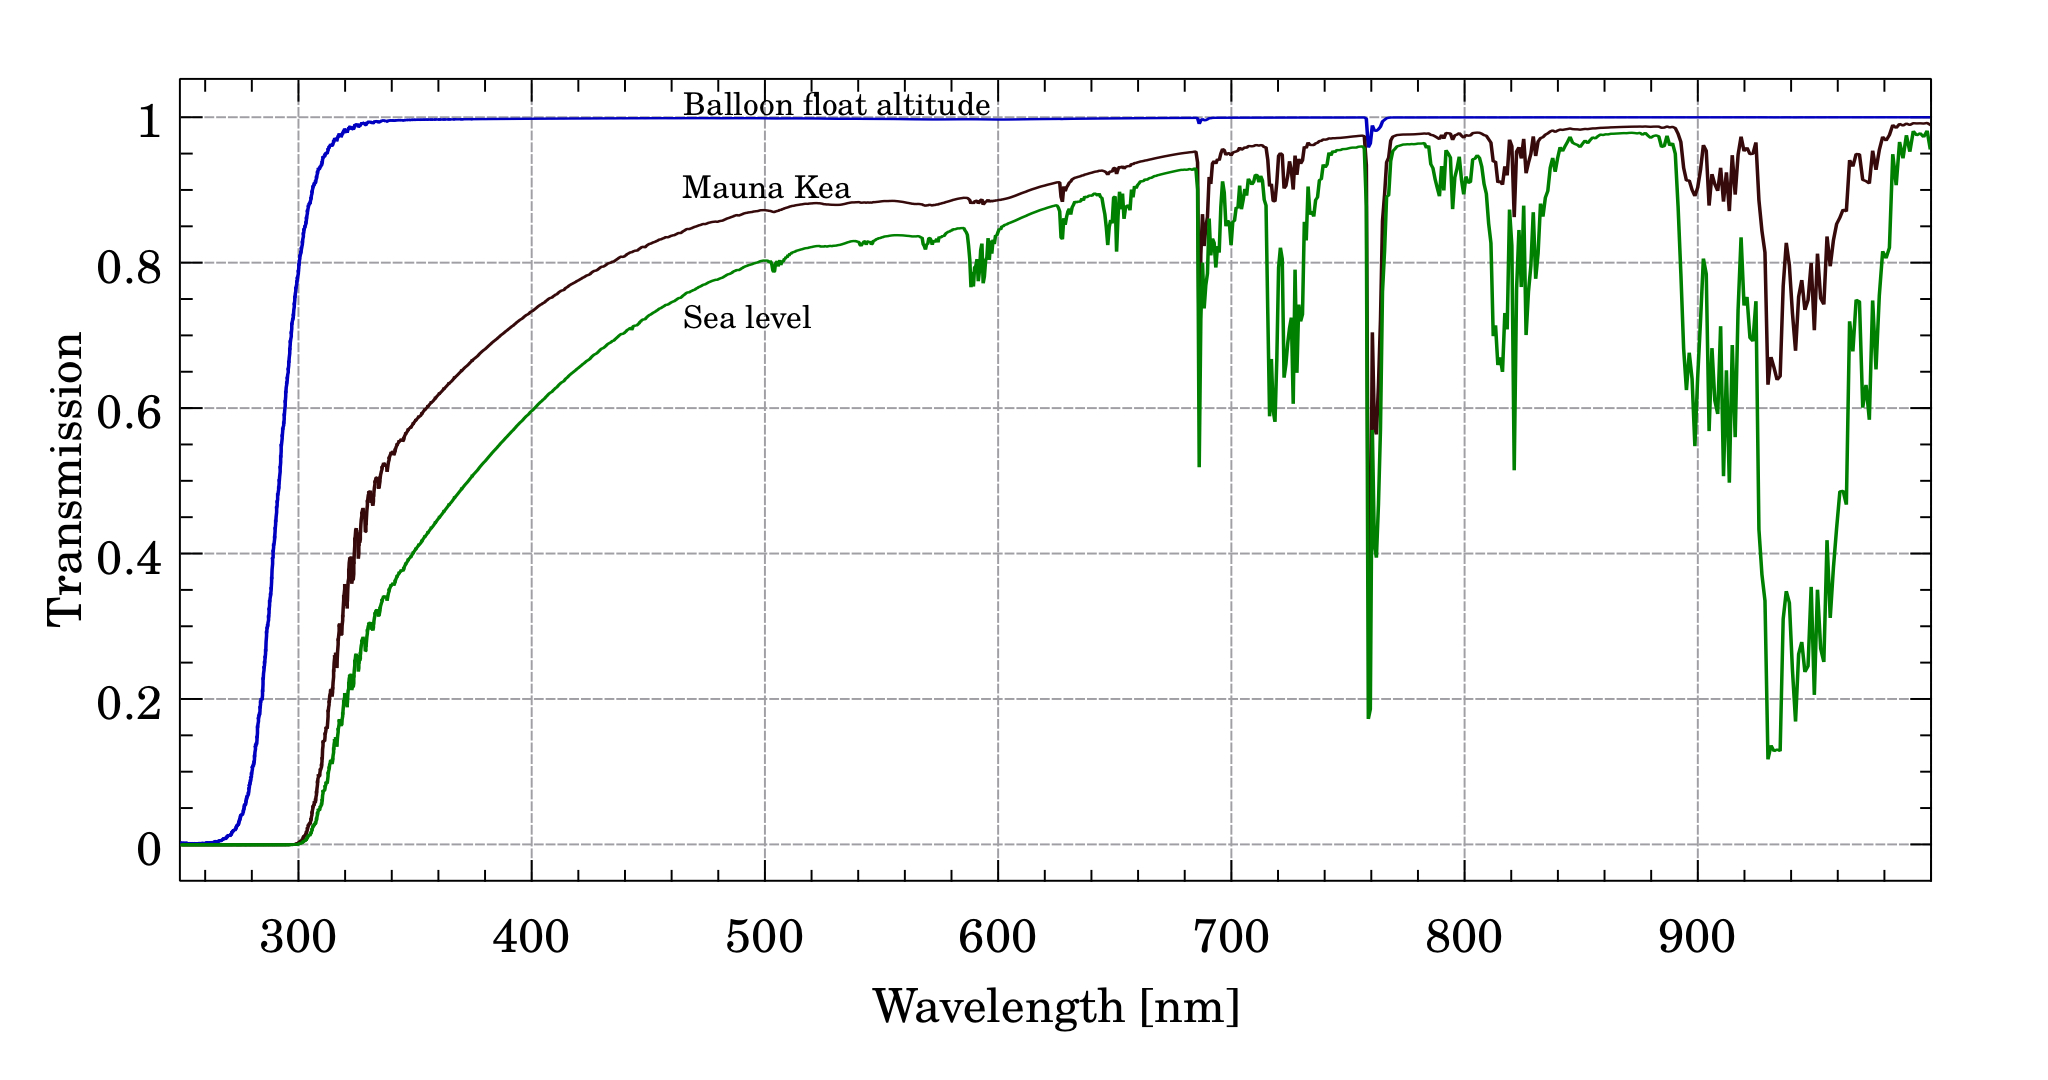
\includegraphics[width=0.95\textwidth]{Introduction/figs/atmosphere.jpg}
        \end{center}
        \caption{Transmission of the atmosphere vs wavelength at sea level (green), Mauna Kea (brown), and balloon float altitude (blue). }
        \label{fig:atmos}
    \end{small}
\end{figure}


\section{Super-pressure Balloon-borne Imaging Telescope (SuperBIT)}
The point of super bit is t be able to provide diffraction limited observations in the near uv and optical. The diffraction limit of the bit sciecne camera is 0.25 arcseconds resolution therefore the stability of the system must be 2 order mags less which leaves us with a goal of 20 milli arcsecond stability this is achieved using two systems. first the gondola which gives a stability of 0.7" and then fgs in the optics that provides further stabliztaion by tip tilt the 100marcsecond. Both systems described in more detail below.
\subsection{The Gondola}
\begin{figure}
    \begin{small}
        \begin{center}
            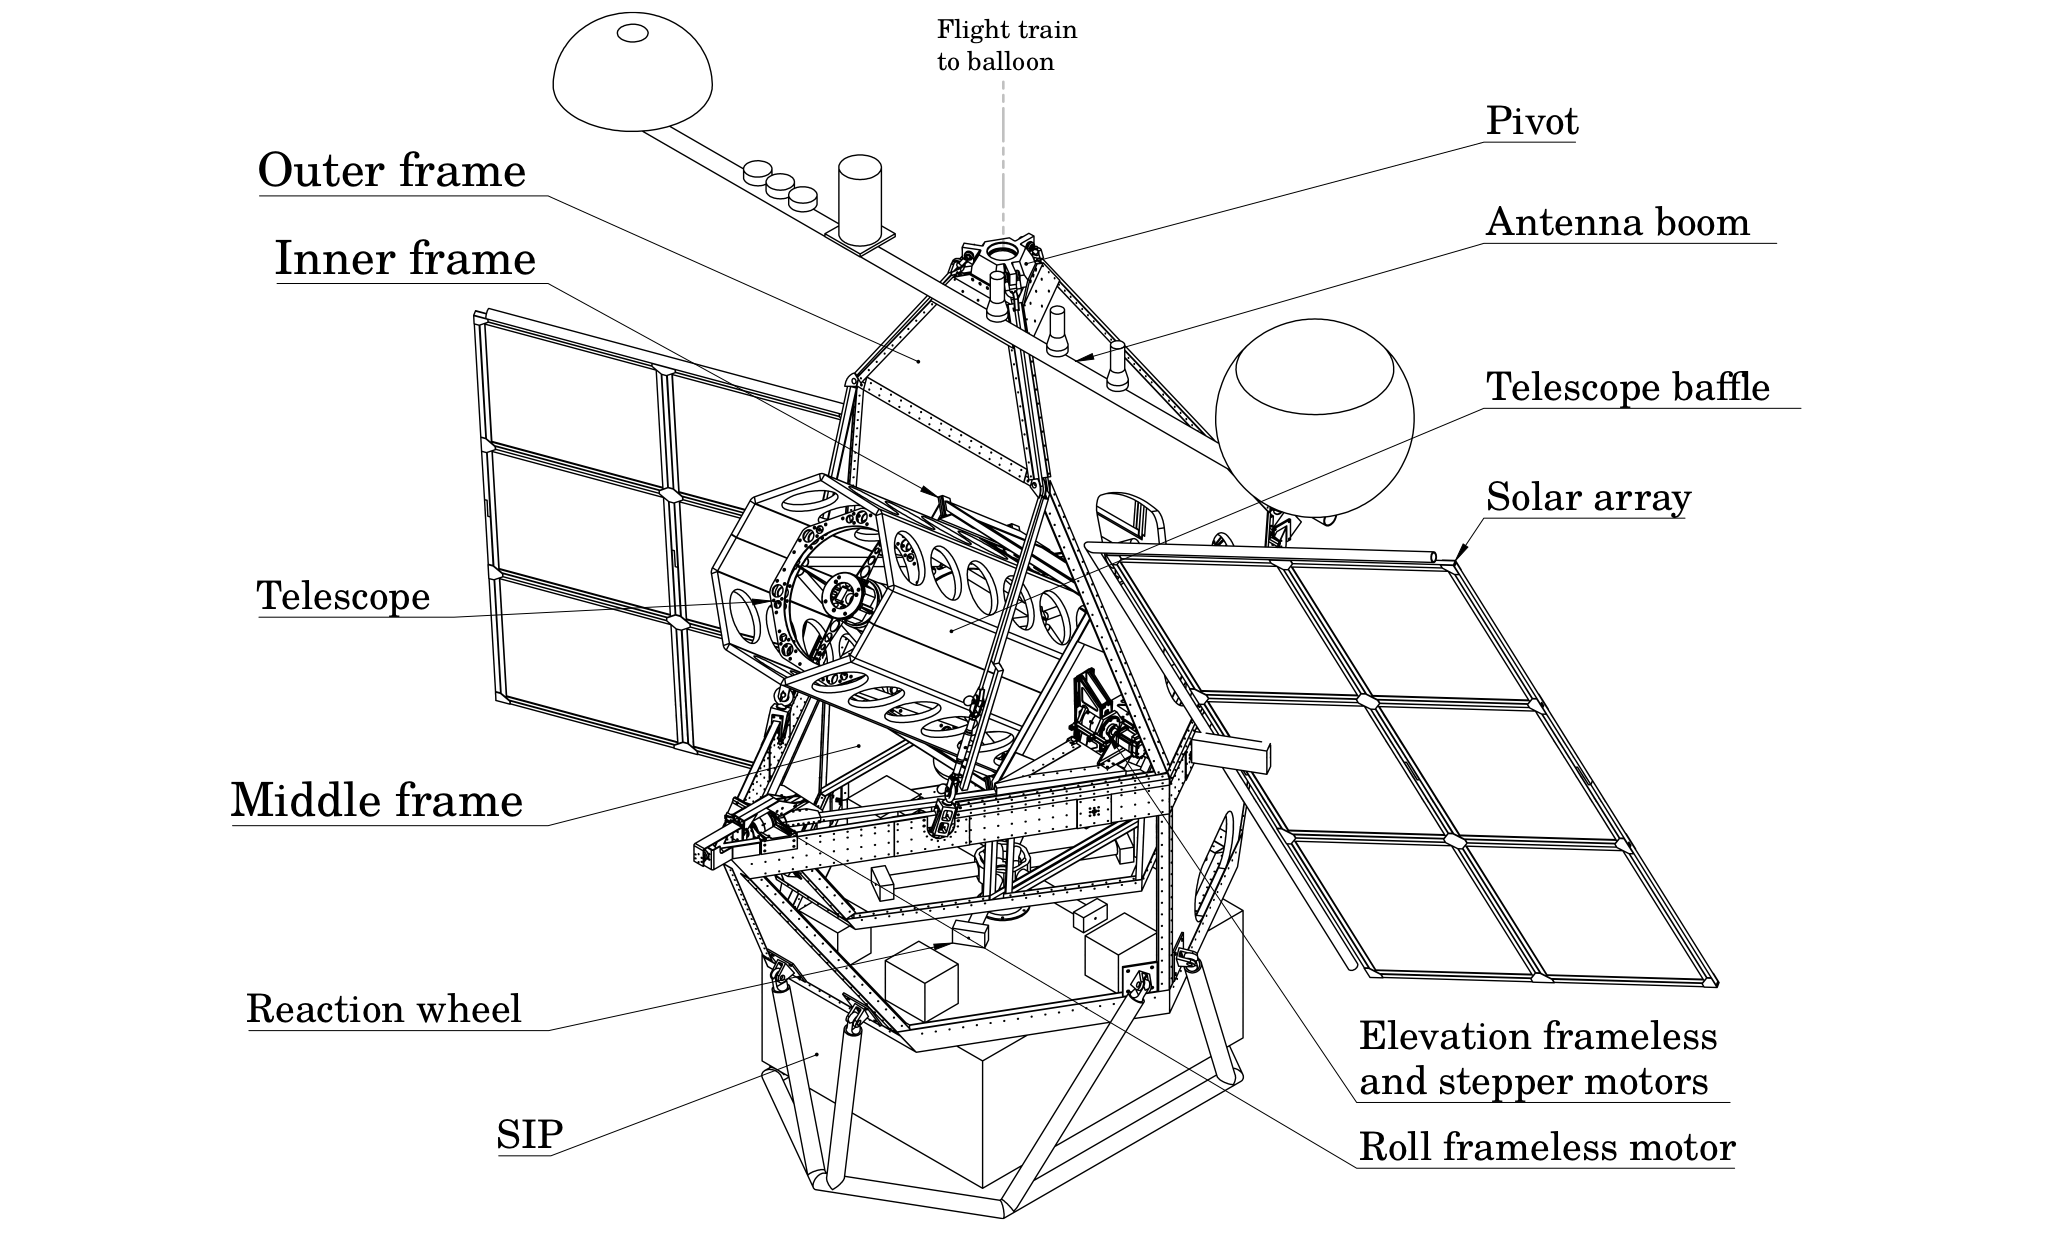
\includegraphics[width=0.95\textwidth]{Introduction/figs/bit_model.png}
        \end{center}
        \caption{Layout of the SuperBIT instrument.}
        \label{fig:bit}
    \end{small}
\end{figure}


\subsection{The Optics}

\begin{figure}
    \begin{small}
        \begin{center}
            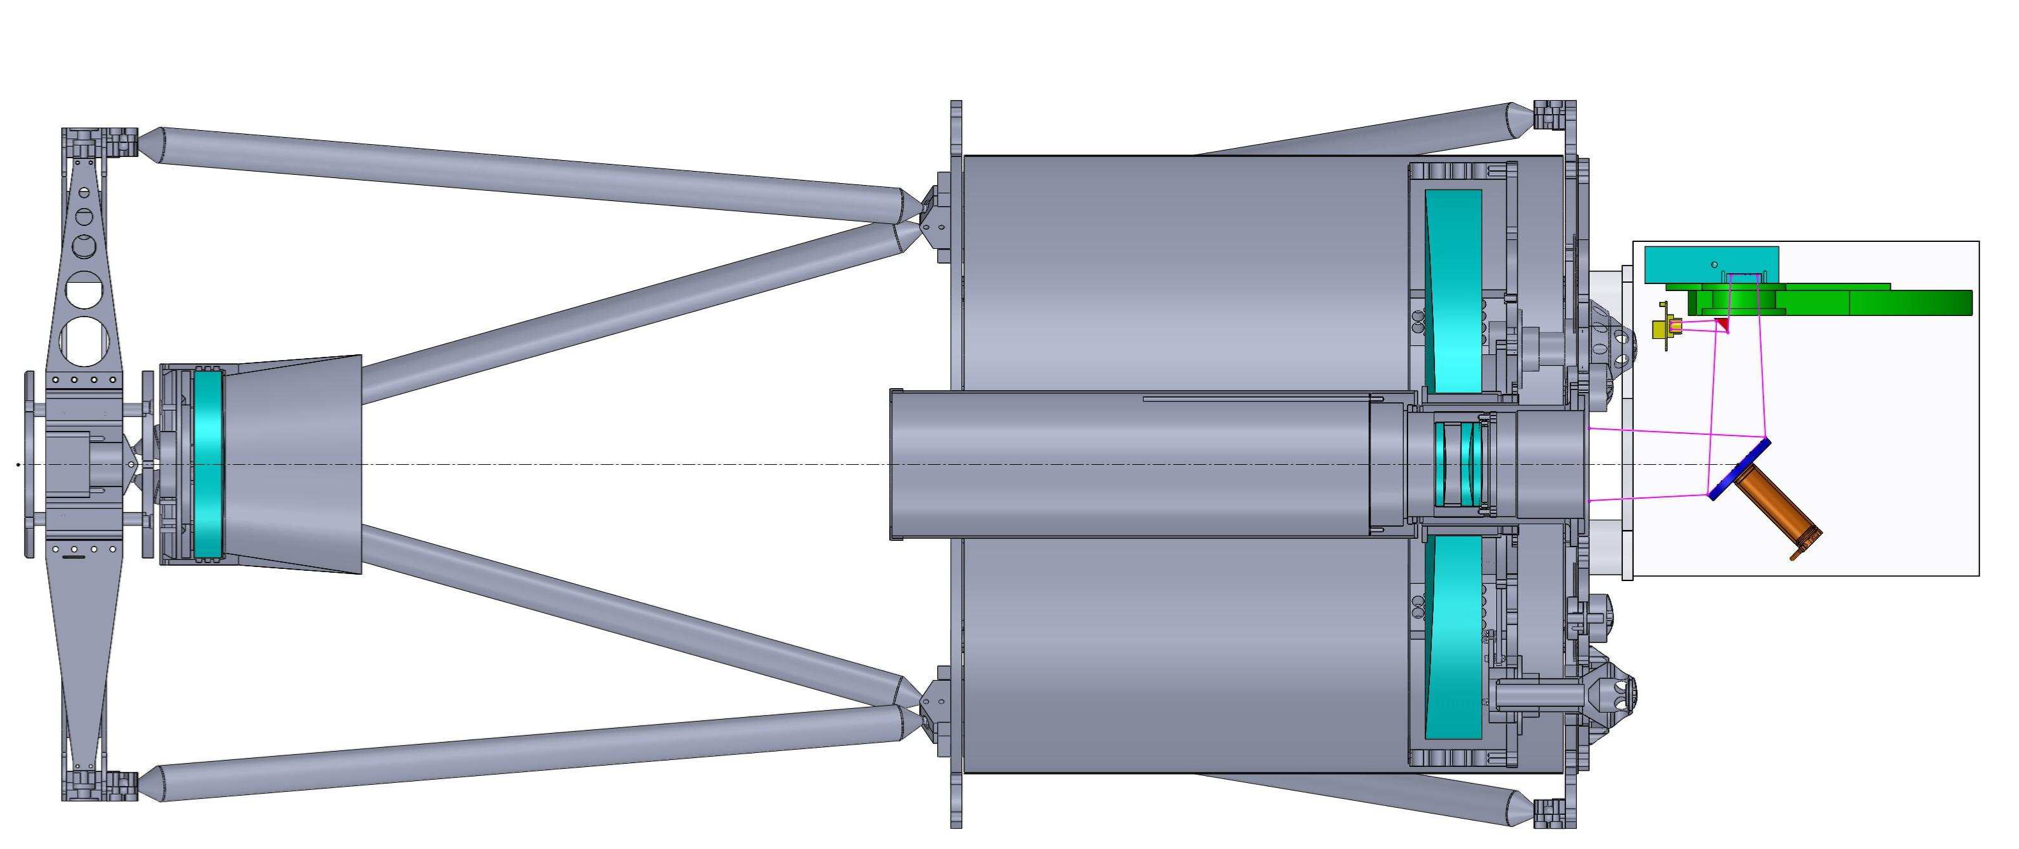
\includegraphics[width=0.95\textwidth]{Introduction/figs/optical_path.png}
        \end{center}
        \caption{The optical layout; The optical path (violet lines) is fed into the fine guidance system through the telescope (grey). The Tip/Tilt mirror (gold and blue) redirects the optical axis 90 degrees to the Science camera (cyan) through a filter wheel (green). Just before the filter wheel some of the light is redirected again by the pick-off mirror (red) to a star camera (yellow).}
        \label{fig:optics}
    \end{small}
\end{figure}

